\chapter{Диаграммы}
\label{cha:design}

В данном разделе производится описание диаграмм, связанных с разработкой распределенной системы фильтрации спама.

\section{Диаграммы использования}
% 
% На рисунке~\ref{fig:usecase1} представлена диаграмма использования системы <<Почтовый Клиент>>.
% 
% \begin{figure}
%   \centering
%   [width=\textwidth]
%   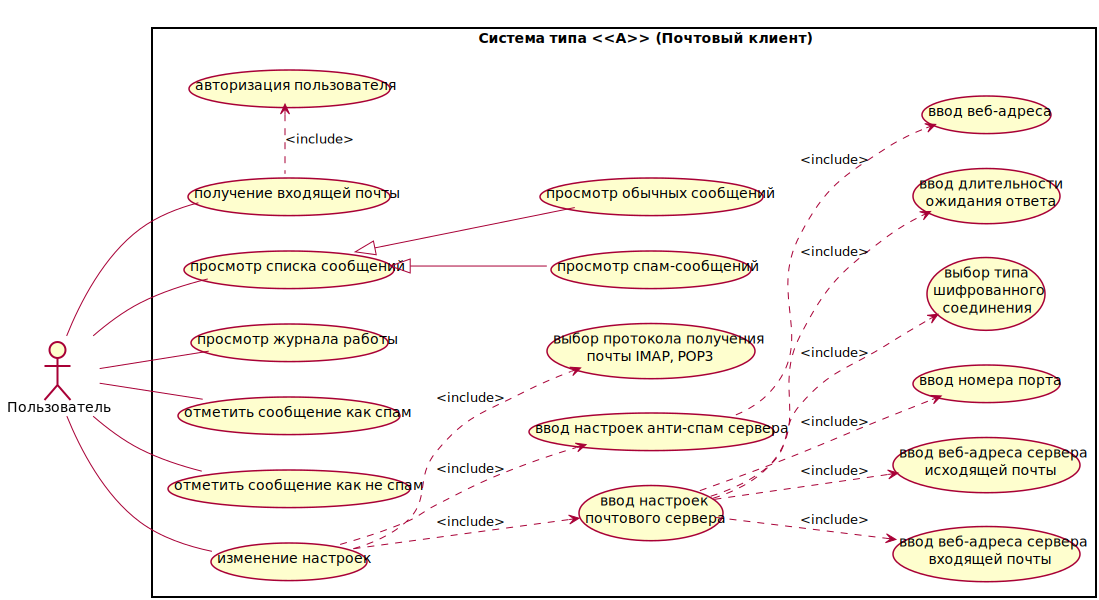
\includegraphics{inc/svg/use-case1}
%   \caption{Диаграмма использования системы <<Почтовый Клиент>>}
%   \label{fig:usecase1}
% \end{figure}
% 
% На рисунке~\ref{fig:usecase2} представлена диаграмма использования системы <<Почтовый Сервер>>.
% 
% \begin{figure}
%   \centering
%   [width=\textwidth]
%   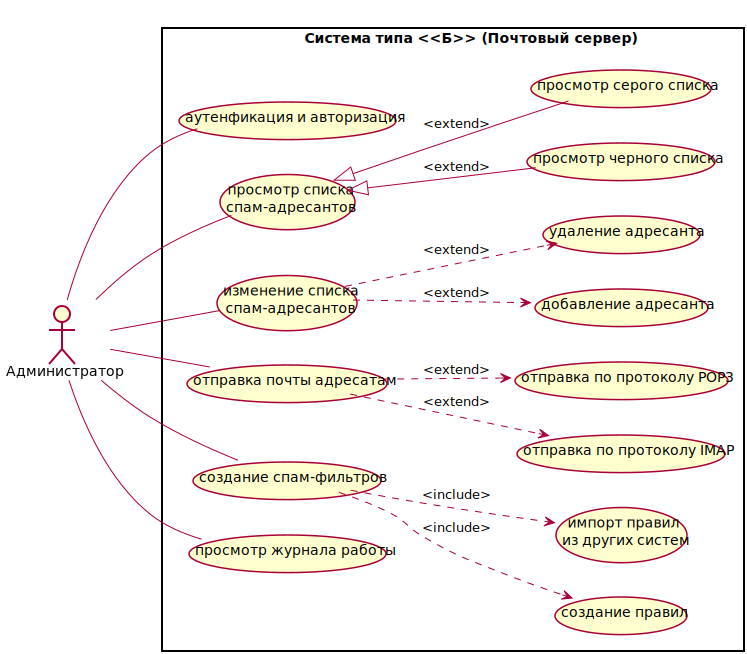
\includegraphics{inc/svg/use-case2}
%   \caption{Диаграмма использования системы <<Почтовый Сервер>>}
%   \label{fig:usecase2}
% \end{figure}
% 
% На рисунке~\ref{fig:usecase3} представлена диаграмма использования системы <<Почтовый Сервер>>.
% 
% \begin{figure}
%   \centering
%   [width=\textwidth]
%   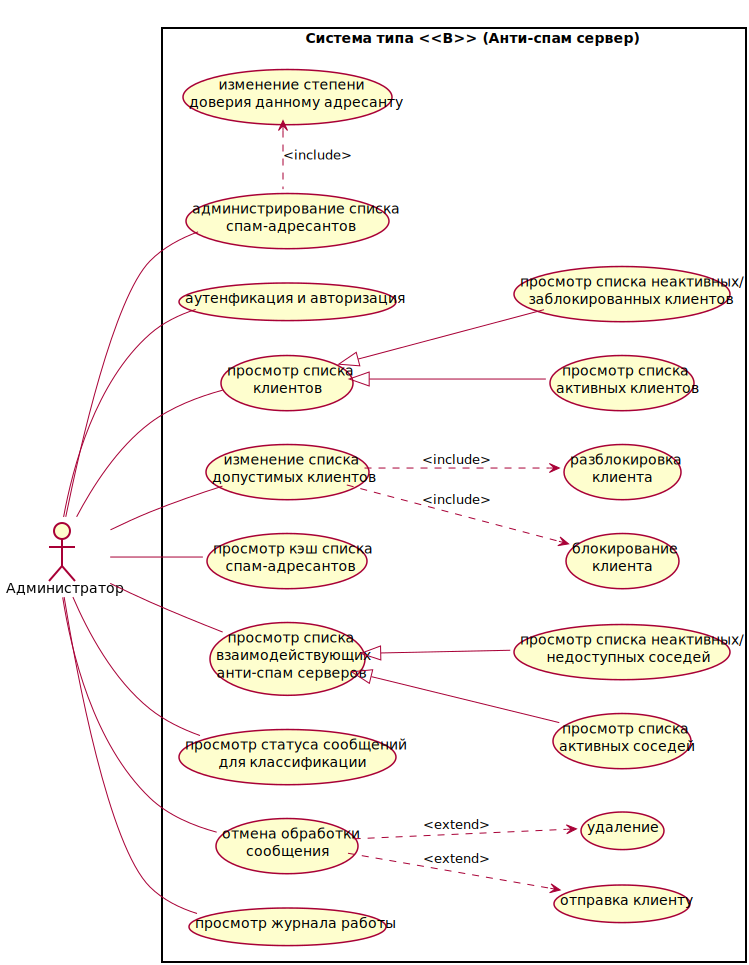
\includegraphics{inc/svg/use-case3}
%   \caption{Диаграмма использования системы <<Анти-спам Сервер>>}
%   \label{fig:usecase3}
% \end{figure}

%\subsection{Блок-схема всякой ерунды}

%\subsubsection*{Кстати о заголовках}

%У нас есть и \Code{subsubsection}. Только лучше её не нумеровать.

%%% Local Variables:
%%% mode: latex
%%% TeX-master: "rpz"
%%% End:
